
%
%%----------------------------------------------------------------


\section{Modelo de información: Módulo Academias}
\subsection{Descripción general}
En la figura~\ref{fig:academias} se muestra la estructura de información que manejará el módulo de academias.

\begin{figure}[htbp!]
	\begin{center}
		\fbox{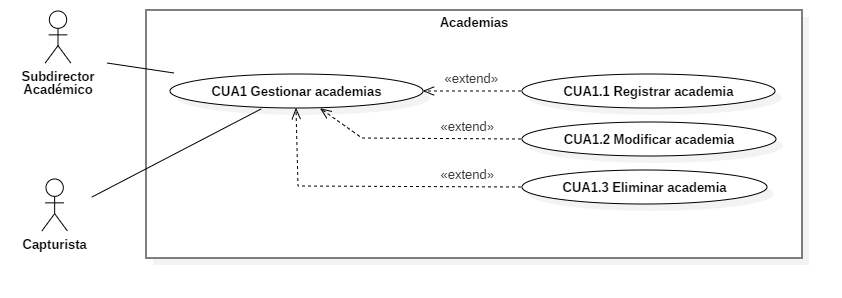
\includegraphics[width=.5\textwidth]{images/clases/Academias.png}}
		\caption{Modelo de información del módulo Academias.}
		\label{fig:academias}
	\end{center}
\end{figure}

%--------------------------------------------------------------------------------
\begin{BusinessEntity}{academia}{Academia}
	
	\Battr{nombre}{Nombre}{\tdFrase}{Es el nombre con el que se registra la academia}{\requerido}{\longitudMax{100}{caracteres}}{Caracteres admitidos: [A-Z] $|$ [a-z] $|$ [á,é,é,ó,ú]  $|$ [Á,É,Í,Ó,Ú] $|$ \textvisiblespace.}

\end{BusinessEntity}


%--------------------------------------------------------------------------------